\documentclass[a4paper]{article}
\usepackage{xeCJK, indentfirst}
\usepackage{amsthm,amssymb,amsmath}
\usepackage{graphicx, subfigure}
\setCJKmainfont{AR PL UMing TW MBE}
\title{火の人工知能玄 Report}
\author{Group 8 鄭余玄、謝昀佐、陳令原}
\date{}
\begin{document}
\maketitle
\section{前言}
這次的 final project 規定是建立一個 Bayesian Belief Network 並且使用 MCMC 方法去解決一個問題。因此我們這組決定跨領域整合,試圖 model 一個真實世界的問題,而不只是能交作業用的 toy problem。2016 年嚴重受到聖嬰現象影響,在新聞報導中時不時會出現森林大火相關報導。此外,森林大火同時也是森林管理一項十分重要的課題,所以我們這組決定以此作為研究主題。

森林大火是一個牽涉很廣泛的問題,如圖\ref{ffp}主要成三部分,分別是森林大火的發生、危害以及後果。研究森林大火的發生成因,需要透過實地田野調查、氣象觀測站、火災數據或相關預報指數等等,收集這些時空資料到 GIS 資料庫中。接著,利用資料所形成的時間和空間機率分布,去訓練出模型進行預測。而此預測的最終目的是,能夠評估火災所帶來的危害,這也是森林大火事件最關心的問題,因為這已經不只影響當地的居民,更擴及到投資人的經濟損失。

\begin{figure}[h]
  \caption{Forest Fire Analysis}
  \centering
  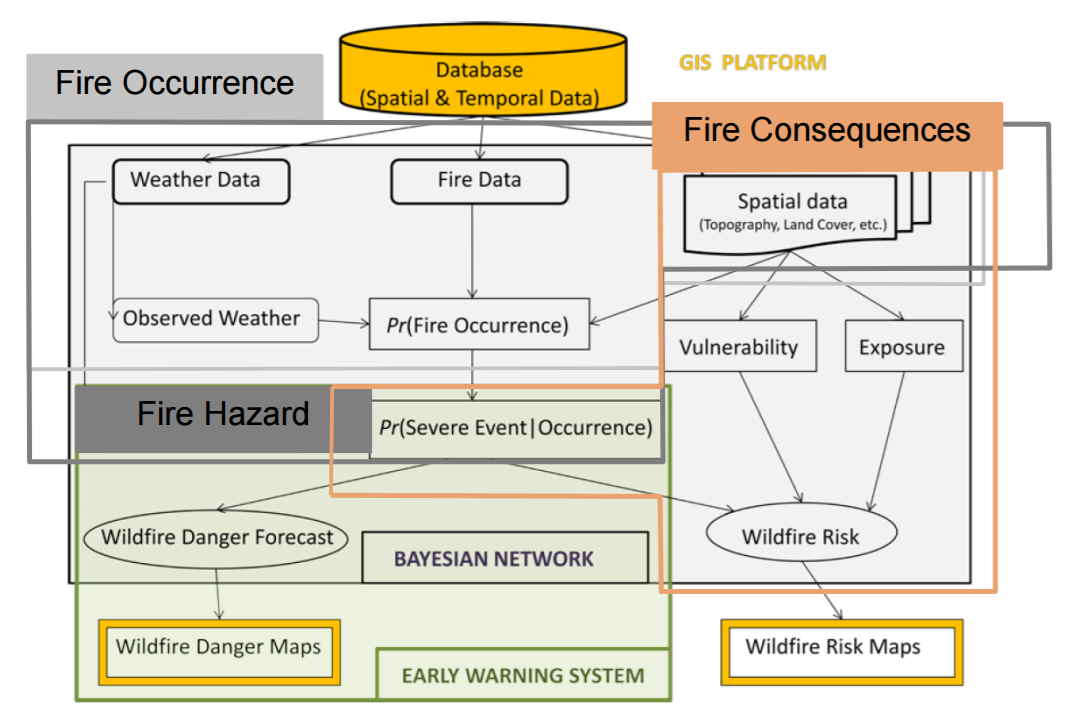
\includegraphics[width=1\textwidth]{problem}
  \label{ffp}
\end{figure}

\section{理論運用}
森林大火的成因分析主要是依據韓國慶州市的一篇研究 \cite{MCFFSK},實地利用異質空間點過程 SPP 去建立森林起火密度模型。再搭配地景、地形起伏、山坡斜率、植被,去進行區域互動共變異影響,建立一個比使用帕松點過程還好的空間邏輯迴歸模型。

繼參考數篇森林大火成因之後,另一篇德國的論文 \cite{BBN}則是討論如何利用這些成因去建立可以自動 structure learning 的 BBN\cite{Model},最後再使用 NBC 去作驗證。這篇論文最終的模型是如圖\ref{bbn_proto},其中目標節點是燃燒面積,而虛線的隨機變數是屬於 hidden variable。

\begin{figure}[h]
  \caption{A BBN model for predicting wildfire spreading}
  \centering
  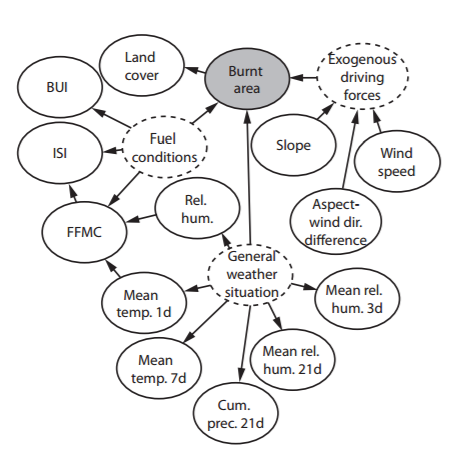
\includegraphics[width=.78\textwidth]{bbn_proto}
  \label{bbn_proto}
\end{figure}

基於實作的可能性,我們將資料簡化,因此資訊的萃取僅採取以FFMC(細小可燃物濕度指數)、DMC(腐植質濕度指數)、DC(乾旱指數)、ISI(初始蔓延速率)、temp(溫度)、RH(相對溼度)、wind(風速)、rain(降雨量)、area(面積)做為一般的隨機變數(random variable),而分別透過DMC、DC生成BUI(累積指數),再由BUI、ISI與FFMC生成Fuel(可燃物指數),以及RH、rain生成Weather(天氣指數)這三個hidden variables,其 BBN 如圖\ref{bbn} 所示。


\begin{figure}[h]
  \caption{BBN}
  \centering
  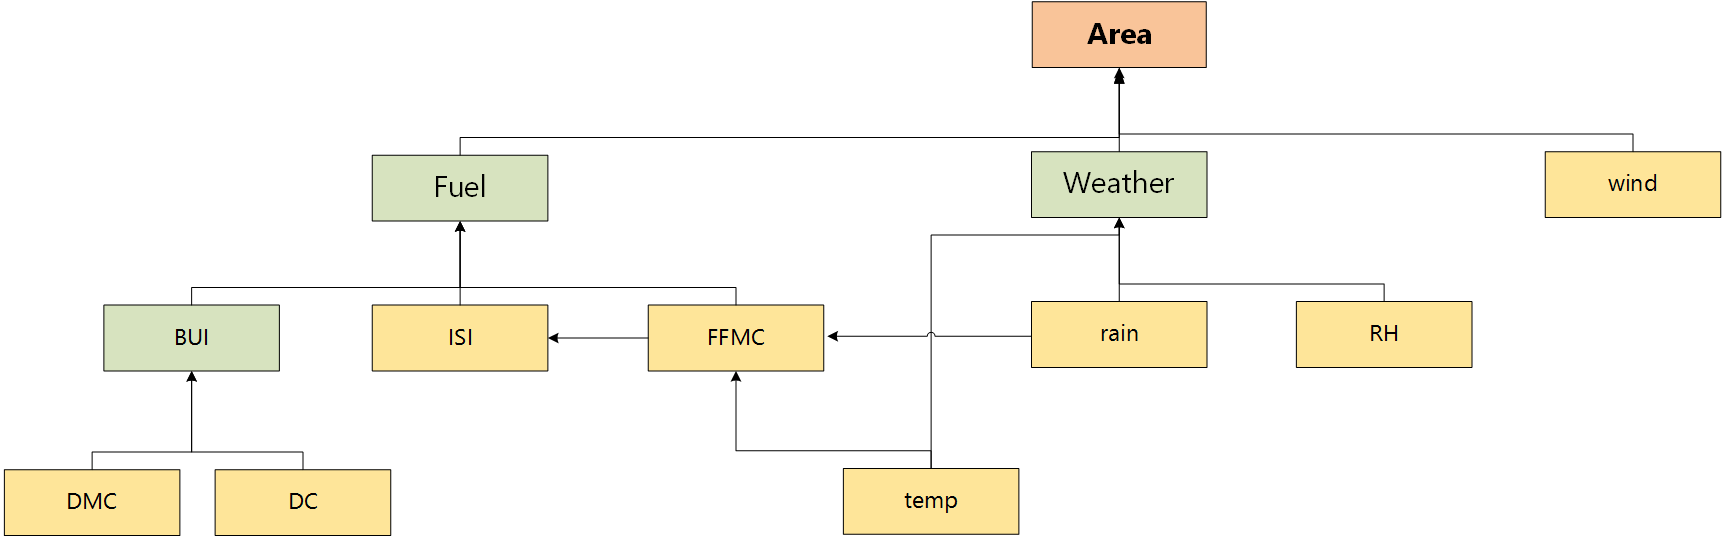
\includegraphics[width=1\textwidth]{bbn}
  \label{bbn}
\end{figure}

\section{實作過程}
因為森林大火我們這組沒有辦法自行蒐集到有效而且完整的資料,所以我們花了需多時間在研究如何形成一個合理並且符合現實情況的模型。我們實作是使用 UCI 機器學習倉儲的森林大火資料集 \cite{UCIFF},接下來的實作步驟是 modal 每個節點,連接這些節點形成 BBN,並且計算出 Conditional Probability Table (CPT),最後使用 MCMC 在機率網路上作 inference。此外,為了驗證程式的正確性,我們有 modal 常見的 rain model,來保證程式碼執行的結果,而且以7:3分配原始資料集作訓練和驗證。

因為這個資料集的燃燒面積偏小,我們推測是因為該地區的植被和降雨量的影響,但是這可能會造成計算時的浮點位數誤差,因此參考使用這個資料集的論文 \cite{dataset},我們一樣使用$\log(X+1)$變換,擴大數值之間的差距如圖\ref{area}。

\begin{figure}[h]
  \caption{Area transformation}
  \centering
  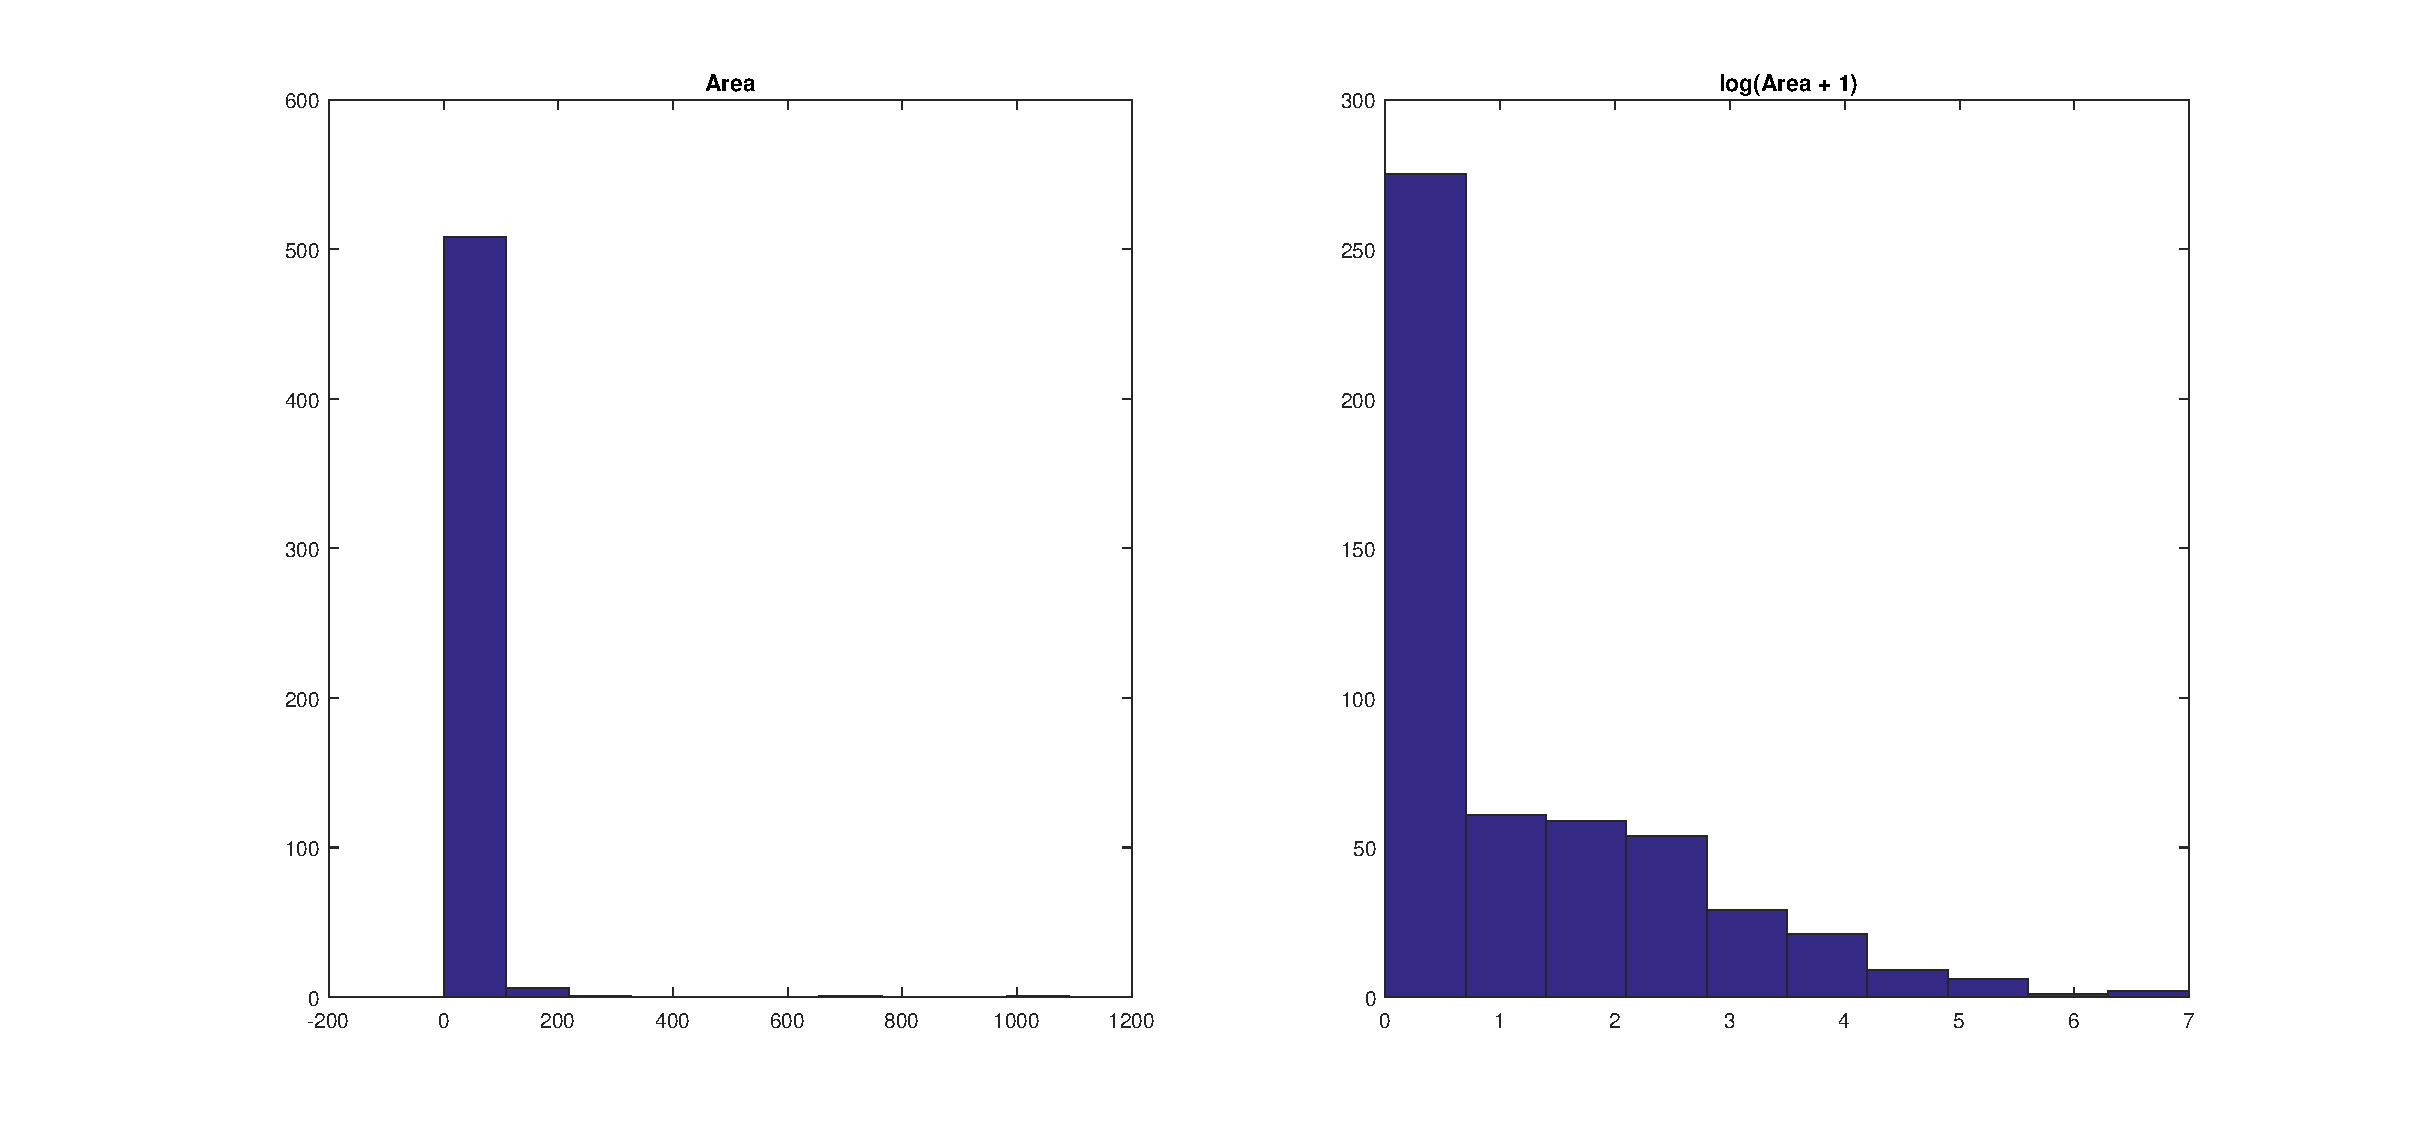
\includegraphics[width=1\textwidth]{area}
  \label{area}
\end{figure}

程式碼的實作,我們參考 The Bayes Net Toolbox for Matlab \cite{bnet},在 MATLAB 上面進行。

\section{實驗}

\section{效能調校}

\bibliographystyle{IEEEtran}
\bibliography{./refs}
\end{document}